\documentclass[letterpaper,10pt, twocolumn]{article}
\usepackage{indentfirst}
\usepackage{listings}
\usepackage{graphicx}
\usepackage{enumitem}
\usepackage{float}
\graphicspath{ {images/} }


\lstset{basicstyle=\ttfamily,
  mathescape=true,
  escapeinside=||}

\begin{document}

\title{\vspace{-2.5cm} \textbf{Attribute Classification: A Varied Approach} \\ \normalsize CS280 Final Project, Spring 2015}
\author{Michelle Nguyen, Allen Tang}
\date{}

\maketitle

\section{Overview}
Human attraction based on physical characteristics translates to a picky phenomenon. Individuals value a wide range of varying attributes, preferring certain facial shapes, hair colors, eye colors, hair lengths, etc. Due to advances in social technology, we are meeting more potential mates more quickly than ever. However, filtering out matches for physical compatibility can be a relatively time-consuming task. 

We use classifiers built upon support vector machines, k-nearest neighbors, and convolutional neural networks\cite{AlexNet} to classify various attributes that are important factors in human attraction. Some of these traits are commonly explored in prior works, such as race and hair color\cite{FaceTracer}. However, our method also allows us to consider more novel features, such as the presence of makeup. These classifiers are then run on "��real-world"�� image sets to create a database of photos that are indexed by attributes. Upon this database, we implement a simple search engine that allows users to easily filter for people of their preferred features. 

\section{Tools}
Most of our preprocessing work, and some classification, was done primarily in Python. Data was collected using the Python Flickr API kit. Face detection was then performed using OpenCV in Python.  K-means and k-NN was ran using the Python package, scikit-learn. For SVM classification, we used LibSVM. Finally, CNNs were implemented in Caffe, running on a GTX 980 GPU.

\section{Dataset}
We created our own datasets using the Flickr API, collecting images based on a set of image tags, i.e. "��asian portrait". By using this versatile method of querying Flickr, we can easily create data for features that have no available dataset online. After pulling these images from Flickr, we had to manually clean our data by removing falsely tagged photos, excessive repeats, grayscale images, bad pose, and more. This constraint required us to generate a reasonably large dataset. This was cumbersome to obtain, but ideally allowed us to generalize our classifiers on a more extensive set of images that capture a wide range of conditions, such as illumination and expression. This ability to generalize is very important given that our ultimate goal is to run our classifier on user-generated images. However, it is important to note that Flickr image data is not completely diverse, as it is heavily biased toward photos of females and certain styles of photos.

After collecting the images, we used the Viola-Jones algorithm in OpenCV to detect faces in the photos. Since one of the attributes we wanted to consider was hair color, we increased the vertical size of the cropped bounding box to include the person's hair as well. Finally, each crop was resized to 100x200.
\begin{figure}
  \centering
    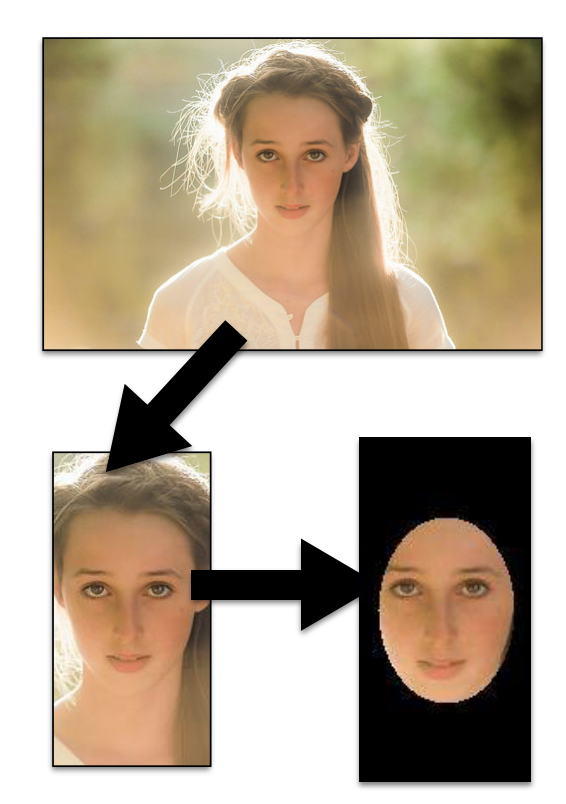
\includegraphics[scale=0.5]{writeup-graphics/processing.png}
  \caption{Steps in processing data}
  \label{fig:facebox}
\end{figure}

For our project, we considered three attributes: race, hair color, and the presence of makeup. 
Our dataset for race consists of four possible categories. For the races Caucasian, Asian, Hispanic, and African we have 1097, 1627, 1124, and 607 images respectively. 
We categorize hair color into three categories, blonde, dark (which includes black and brown), and red. For these categories, we have 572, 915, and 415 photos respectively.
Finally, the problem of detecting the presence of makeup is a binary classification. We have 709 images of people with no makeup and 946 images of people with makeup.
We used $20\%$ of our images as our test set.

\section{Feature Classification}
We classified three different attributes: race, hair color, and presence of makeup using several classifiers.
\subsection{SVM}
Our first approach was to classify race using a SVM with a linear kernel. We tried a variety of techniques to standardize the images:
\begin{enumerate}[topsep=5pt,itemsep=1ex,partopsep=0ex,parsep=0ex]
\item No change
\item Normalization to mean 0 and unit variance
\item Normalization by dividing image mean
\end{enumerate}
We denote the above as 'config' in our results section.\\

We also experimented with using the raw pixel values versus converting the image to grayscale. Then, we applied a Gaussian blur with $\sigma=.7$, and applied a specific mask which gave us the face and hair. We experimented with parameters and found $c=0.05$ gave us best results. 

\subsection{k-means/k-NN}
For the attribute of hair color, we tried an approach involving both k-means and k-NN. We first applied a mask to each image to extract the hair at the top of the person'��s head. After applying the mask, we used k-means and vector quantization to find the most dominant color in that image region. The RGB values for that dominant color were used as the feature vector for that image in k-NN. By doing so, we could determine the label for an image by taking the most common label for images with similar colors. From our predictions, we found that using a large number of neighbors kept us from overfitting. We determined that our best value of k was 300.
\begin{figure}[H]
  \centering
    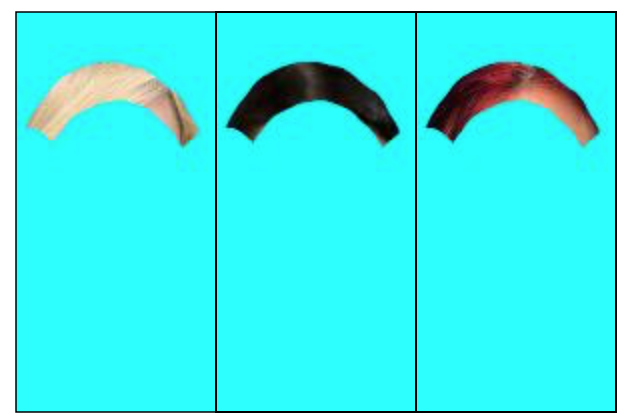
\includegraphics[scale=0.5]{writeup-graphics/haircrops.png}
  \caption{Examples of masked hair. A cyan background was used to distinguish from black hair in the k-means step.}
  \label{fig:facebox}
\end{figure}

\subsection{CNN}
CNN was used as a classifier for all three attributes. Before sending the images through our neural network, we first resized our photos to a size of 227 x 227.
Then, we attempted a variety of CNN architectures, each trained for 10,000 iterations. Our most successful neural networks were:
\begin{enumerate}[topsep=5pt,itemsep=1ex,partopsep=0ex,parsep=0ex]
\item AlexNet with Softmax
\item Modified AlexNet, with convolutional layers 3, 4 removed with Softmax
\item Modified AlexNet, with convolutional layers 3, 4, as well as fc6, relu6, and drop6 removed with Softmax
\end{enumerate}
We denote the above as 'config' in our results section.\\
\section{Results}
\subsection{Race}
\begin{figure}[H]
  \centering
    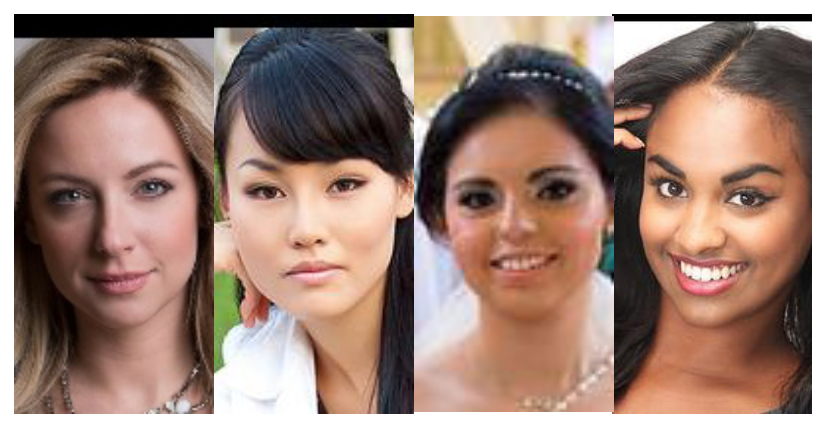
\includegraphics[scale=0.5]{writeup-graphics/races.png}
  \caption{Examples of training data for each race}
  \label{fig:facebox}
\end{figure}
We found that training a CNN on our race dataset gave slightly better results than those that we got from training a SVM. This was no surprise, and is likely due to all the variance in our dataset, which CNN is more robust against. \\
Surprisingly, when running a CNN on our dataset without masking for faces, we obtained an accuracy of 74.9\%. This is not much worse than training the CNN on the masked version of the data, which gave us an accuracy of 76.2\%. \\
Finally, we found that despite the limited amount of training data we had, the full implementation AlexNet gave us the best results over the simpler networks that we attempted.
\begin{table}[H]
\caption{Linear SVM, config=3, c=0.05, facemask} % title of Table
\centering % used for centering table
\begin{tabular}{c c c c} % centered columns (4 columns)
\hline\hline %inserts double horizontal lines
Race & Precision & Recall & Samples \\ [0.5ex] % inserts table
%heading
\hline % inserts single horizontal line
Caucasian & 0.69 & 0.69 & 219 \\ % inserting body of the table
Asian & 0.62 & 0.62 & 325 \\
Hispanic & 0.81 & 0.81 & 225 \\
African & 0.93 & 0.93 & 121 \\[1ex] % [1ex] adds vertical space
\hline %inserts single line
 & MAP & Accuracy\\
\hline
Total & 0.76 & 0.73 & 890 \\
\end{tabular}
\label{table:nonlin} % is used to refer this table in the text
\end{table}

\begin{table}[H]
\caption{CNN, config=1, facemask} % title of Table
\centering % used for centering table
\begin{tabular}{c c c c} % centered columns (4 columns)
\hline\hline %inserts double horizontal lines
Race & Precision & Recall & Samples \\ [0.5ex] % inserts table
%heading
\hline % inserts single horizontal line
Caucasian & 0.73 & 0.73 & 219 \\ % inserting body of the table
Asian & 0.73 & 0.68 & 325 \\
Hispanic & 0.82 & 0.83 & 225 \\
African & 0.75 & 0.89 & 121  \\[1ex] % [1ex] adds vertical space
\hline %inserts single line
 & MAP & Accuracy\\
\hline
Total & 0.76 & 0.76 & 890 \\
\end{tabular}
\label{table:nonlin} % is used to refer this table in the text
\end{table}

\subsection{Hair Color}
For hair color, we tried using k-NN and CNN as our classifiers. For k-NN with a large number of neighbors, we were able to obtain reasonable results which gave us 76.7\% accuracy. Training a CNN on images with a mask for hair gave us even better results at 80.9\% accuracy. For both classifiers, we see it is easier to distinguish red hair from the other two categories. However, training CNN on images without the mask was not as successful and gave numbers that hovered around a 60\% accuracy. \\
Overall, we found our outcome surprisingly successful despite the high variance in the photos for lighting, pose, and hairstyle.
\begin{table}[H]
\caption{k-means/k-NN[k=400], hairmask} % title of Table
\centering % used for centering table
\begin{tabular}{c c c c} % centered columns (4 columns)
\hline\hline %inserts double horizontal lines
Color & Precision & Recall & Samples \\ [0.5ex] % inserts table
%heading
\hline % inserts single horizontal line
Blonde & 0.68 & 0.74 & 114 \\ % inserting body of the table
Dark & 0.77 & 0.72 & 183 \\
Red & 0.90 & 0.92 & 83 \\[1ex] % [1ex] adds vertical space
\hline %inserts single line
 & MAP & Accuracy\\
\hline %inserts single line
Total & 0.78 & 0.77 & 380\\
\hline
\end{tabular}
\label{table:nonlin} % is used to refer this table in the text
\end{table}

\begin{table}[H]
\caption{CNN, config=1, hairmask} % title of Table
\centering % used for centering table
\begin{tabular}{c c c c} % centered columns (4 columns)
\hline\hline %inserts double horizontal lines
Color & Precision & Recall & Samples \\ [0.5ex] % inserts table
%heading
\hline % inserts single horizontal line
Blonde & 0.74 & 0.82 & 114 \\ % inserting body of the table
Dark & 0.81 & 0.76 & 183 \\
Red & 0.90 & 0.92 & 83 \\[1ex] % [1ex] adds vertical space
\hline %inserts single line
 & MAP & Accuracy\\
\hline %inserts single line
Total & 0.82 & 0.81 & 380\\
\hline
\end{tabular}
\label{table:nonlin} % is used to refer this table in the text
\end{table}

\subsection{Makeup}
\begin{figure}
  \centering
    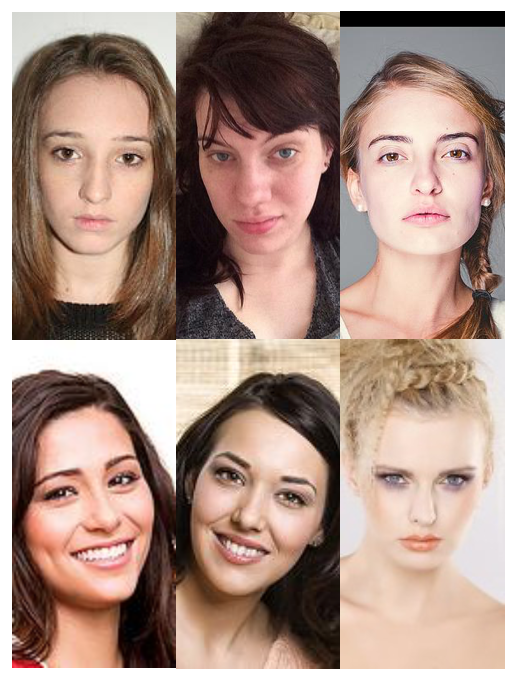
\includegraphics[scale=0.5]{writeup-graphics/makeup.png}
  \caption{Faces with no makeup (top) versus with makeup (bottom)}
  \label{fig:facebox}
\end{figure}
Finally, we trained a CNN for our binary classification problem of detecting the presence of makeup on a person's face. This gave us an accuracy of 82.5\%. Although makeup can often be very subtle, such as simple eyeliner and mascara, these numbers are promising. 

\begin{table}[H]
\caption{CNN, config=1, unmasked} % title of Table
\centering % used for centering table
\begin{tabular}{c c c c} % centered columns (4 columns)
\hline\hline %inserts double horizontal lines
Race & Precision & Recall & Samples \\ [0.5ex] % inserts table
%heading
\hline % inserts single horizontal line
Yes & 0.76 & 0.89 & 142 \\ % inserting body of the table
No & 0.90 & 0.78 & 189 \\[1ex] % [1ex] adds vertical space
\hline %inserts single line
 & MAP & Accuracy\\
\hline %inserts single line
Total & 0.83 & 0.83 & 331\\
\hline
\end{tabular}
\label{table:nonlin} % is used to refer this table in the text
\end{table}

\section{Search Engine}

\begin{figure}
  \centering
    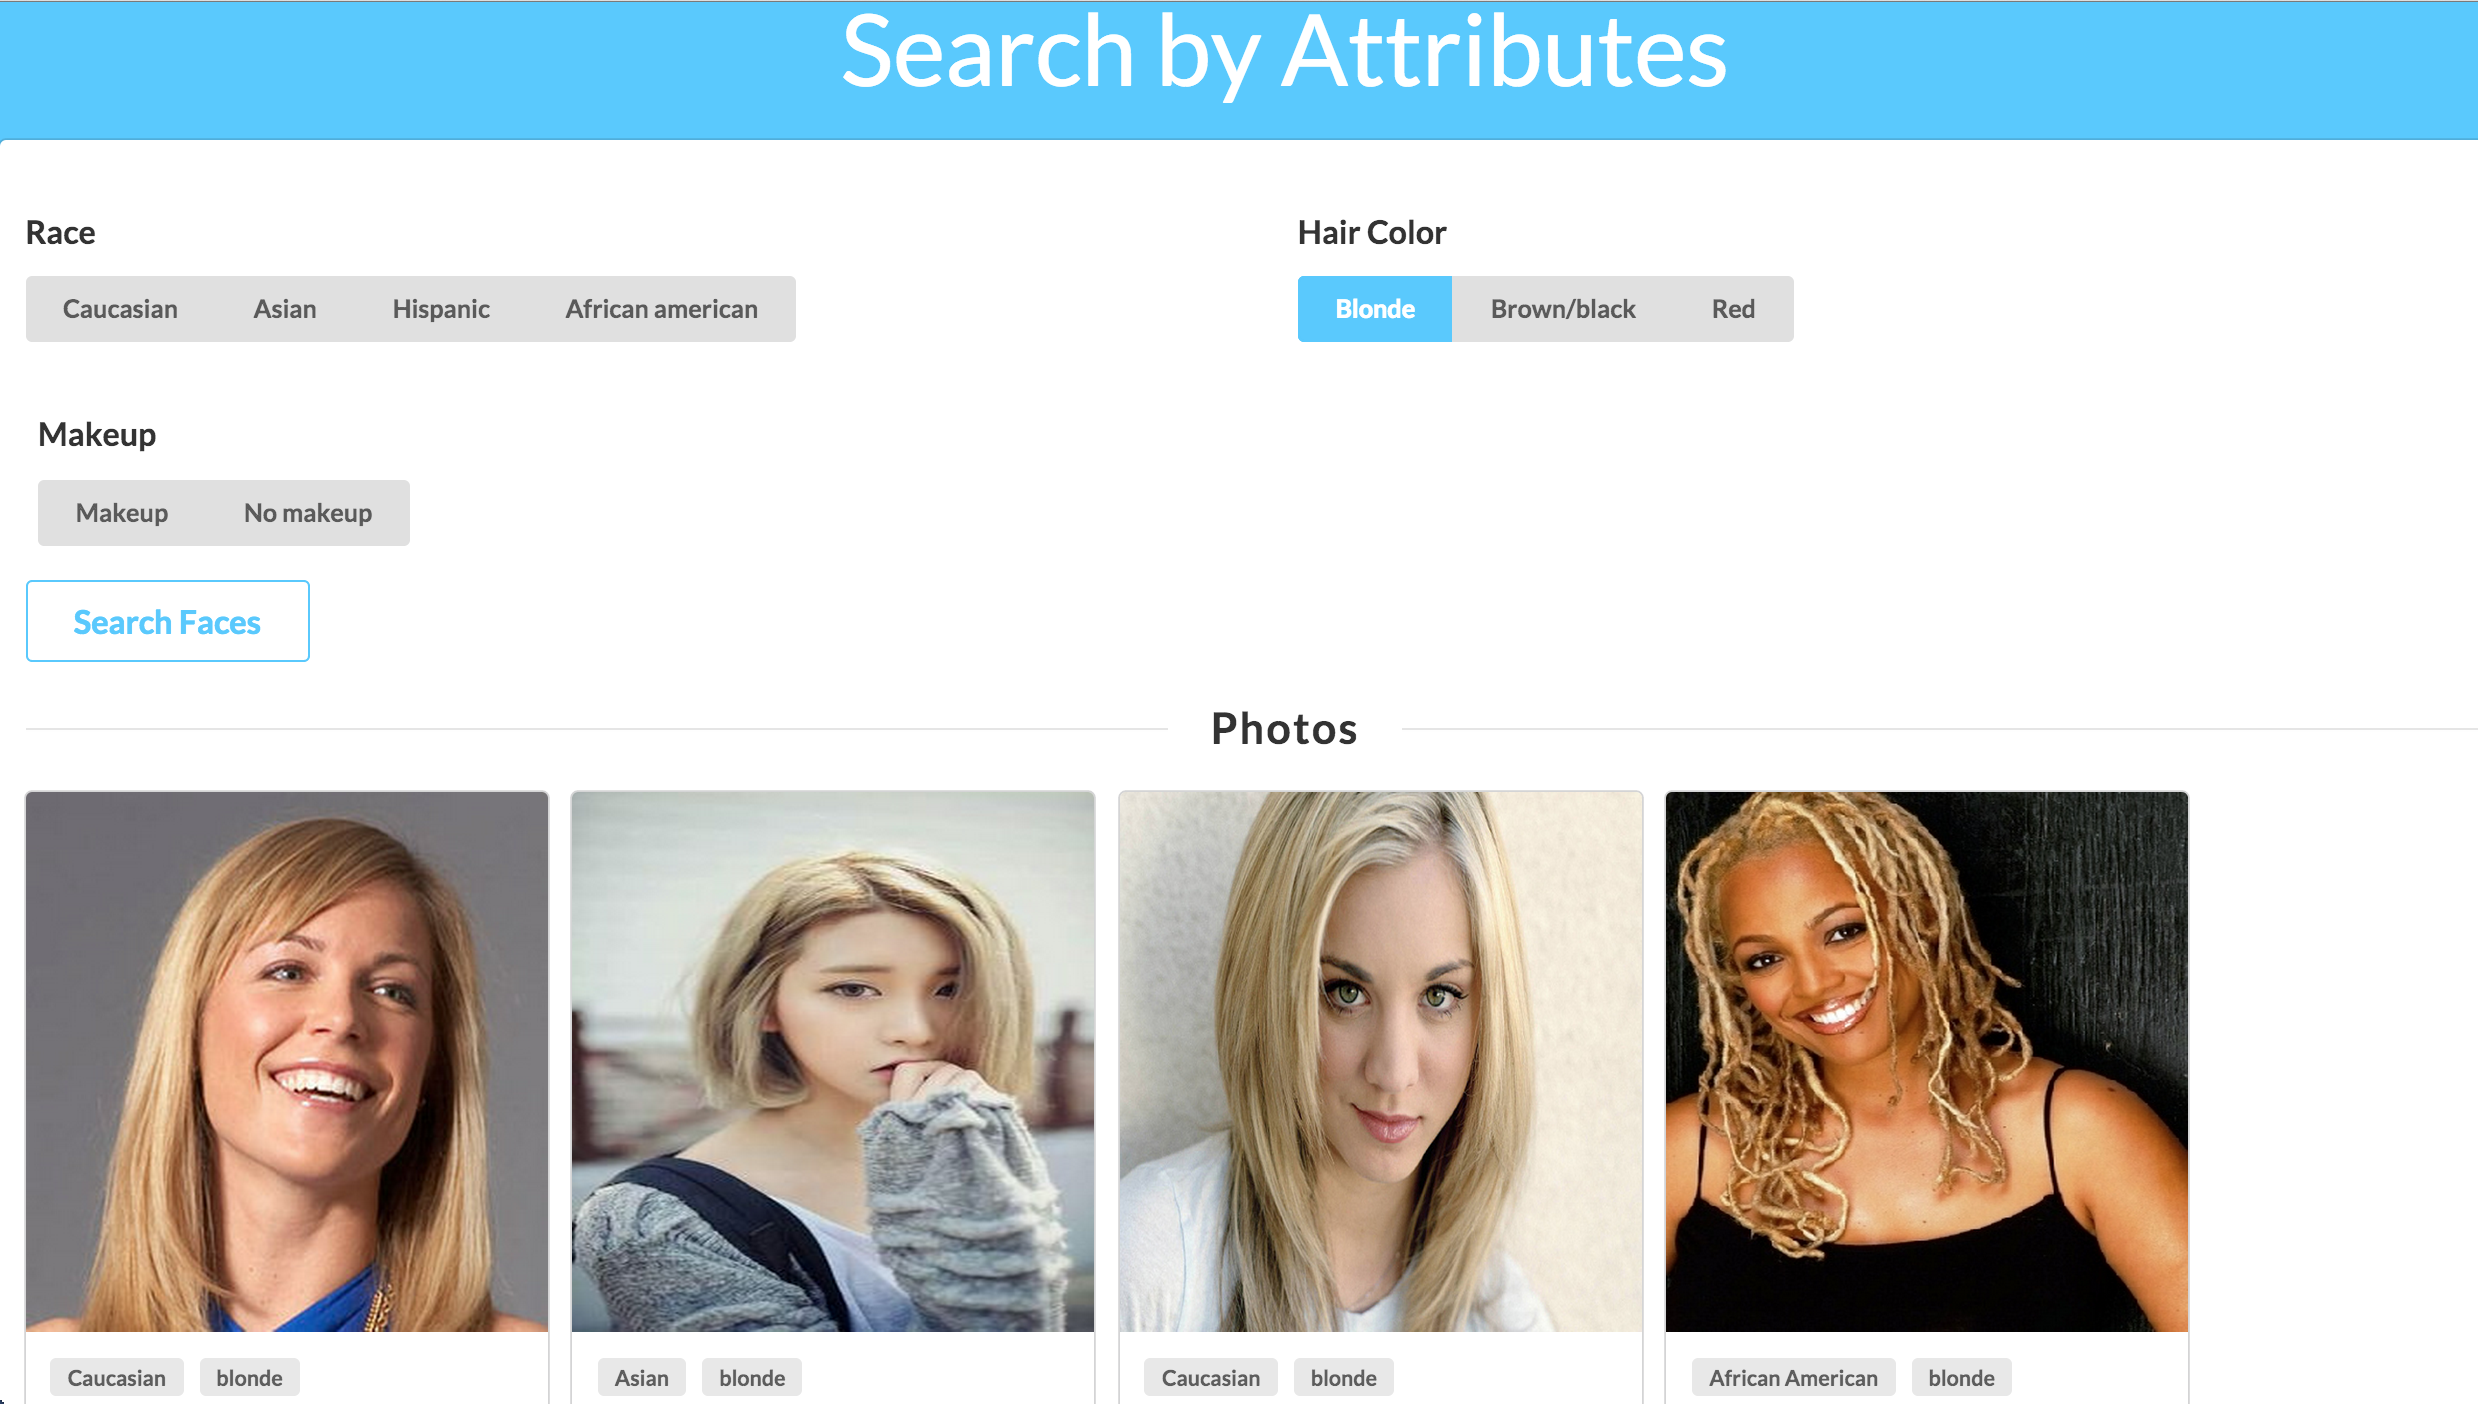
\includegraphics[scale=0.2]{writeup-graphics/website.png}
  \caption{The Attribute Search frontend}
  \label{fig:facebox}
\end{figure}
 \textbf{http://attributesearch.herokuapp.com}\\ 
 
We then collected images by using the Flickr API with search queries that did not correspond to any of our attribute categories. For instance, we pulled images from Flickr corresponding to the generic tag, "��portrait"��. Then, with the best classifiers for each of our attributes, we classified each image and stored them with their corresponding categories in a PostgreSQL database.

Upon the database, we built a simple search engine using Ruby on Rails. This search engine idea is similar to the search engine created by Kumar et al. The search engine allows users to filter for attributes for a set of images that have been categorized by our classifiers. The images are displayed along with tags showing what attributes the photo'��s subject has.

\section{Conclusion}
Although our results, given our limited dataset, were not as good as those obtained via the region-specific SVMs by Kumar et. al, we have shown that neural networks can provide a decent framework for general classification problems involving attributes. We were able to get close to 0.75 accuracy or above on a wide range of attribute problems with an almost off-the-shelf implementation of AlexNet. In contrast, our semi off-the-shelf SVM approach gave decent results, but certainly required more tuning.

Obtaining good data from Flickr was very challenging and tedious. Resorting to using Amazon Mechanical-Turk would have certainly helped in this regard. Due to these constraints, we were forced to run our classifier on a smaller dataset (orders of magnitude smaller in size than those used in previous approaches) than we would have liked. Due to our own human error, these datasets may also be slightly noisy as well. However, even so, we were able to get promising results. With an even larger and cleaner dataset, predictions may be even more accurate.
\section{Future Work}
There is certainly a possibility that well-tuned neural networks may eventually achieve results comparable to state-of-the-art approaches using region-based SVMs. To do this however, will likely require a very large, accurately-labeled, and diverse dataset. This area would certainly be of interest for future work.

Another topic to consider is the exploration of even more novel attributes. Some traits we had wanted to tackle were eye color, which is feasible with Flickr's high resolution photos, and detecting whether the photo's subject had dimples.






\begin{thebibliography}{9}
\bibitem{AlexNet}
A. Krizhevsky, I. Sutskever, and G. Hinton. ImageNet classification with deep convolutional neural networks. In NIPS, 2012.
\bibitem{FaceTracer}
	N. Kumar, P. N. Belhumeur, and S. K. Nayar. 
	FaceTracer: A Search Engine for Large Collections of Images with Faces. In
	European Conference on Computer Vision (ECCV), 
	pp.340-353, Oct, 2008.
\bibitem{LeCun}
	P. Sermanet, K. Kavukcuoglu, S. Chintala, and Y. LeCun. Pedestrian
	detection with unsupervised multi-stage feature learning. In CVPR,
	2013.


\end{thebibliography}
\end{document}
